\section{Participation notes 1}
Participant: Professional.

\begin{itemize}
    \item \textbf{Have them read the code-example} -  Participant did not have any problem reading the code.
    \item \textbf{Have them draw the structure} - The participant started with drawing the execution flow of the main function using a circle and called it "start", then added two boxes and said this was the two functions side the "World" namespace and drew an arrow from main to the first function main called, then from that function to the second function. Then from the second function to a circle named "end". After this it was mentioned to visualize the "World" namespace, the participant drew a box surrounding the two functions within it and called it "World" at first but then shifted this to be the "std" namespace and draw another namespace box around the whole visualization and called it "World".
    \item \textbf{Have them submit the git URL} - URL submission went without problem and seemed to be intuitive although the participant used the cached input on the URL field and did not type it fully.
    \item \textbf{Have them get the main() implementation} - Participant was able to find implementation of main. Participant wasn't able to find the implementation of the other functions.
    \item \textbf{Participant visualization} 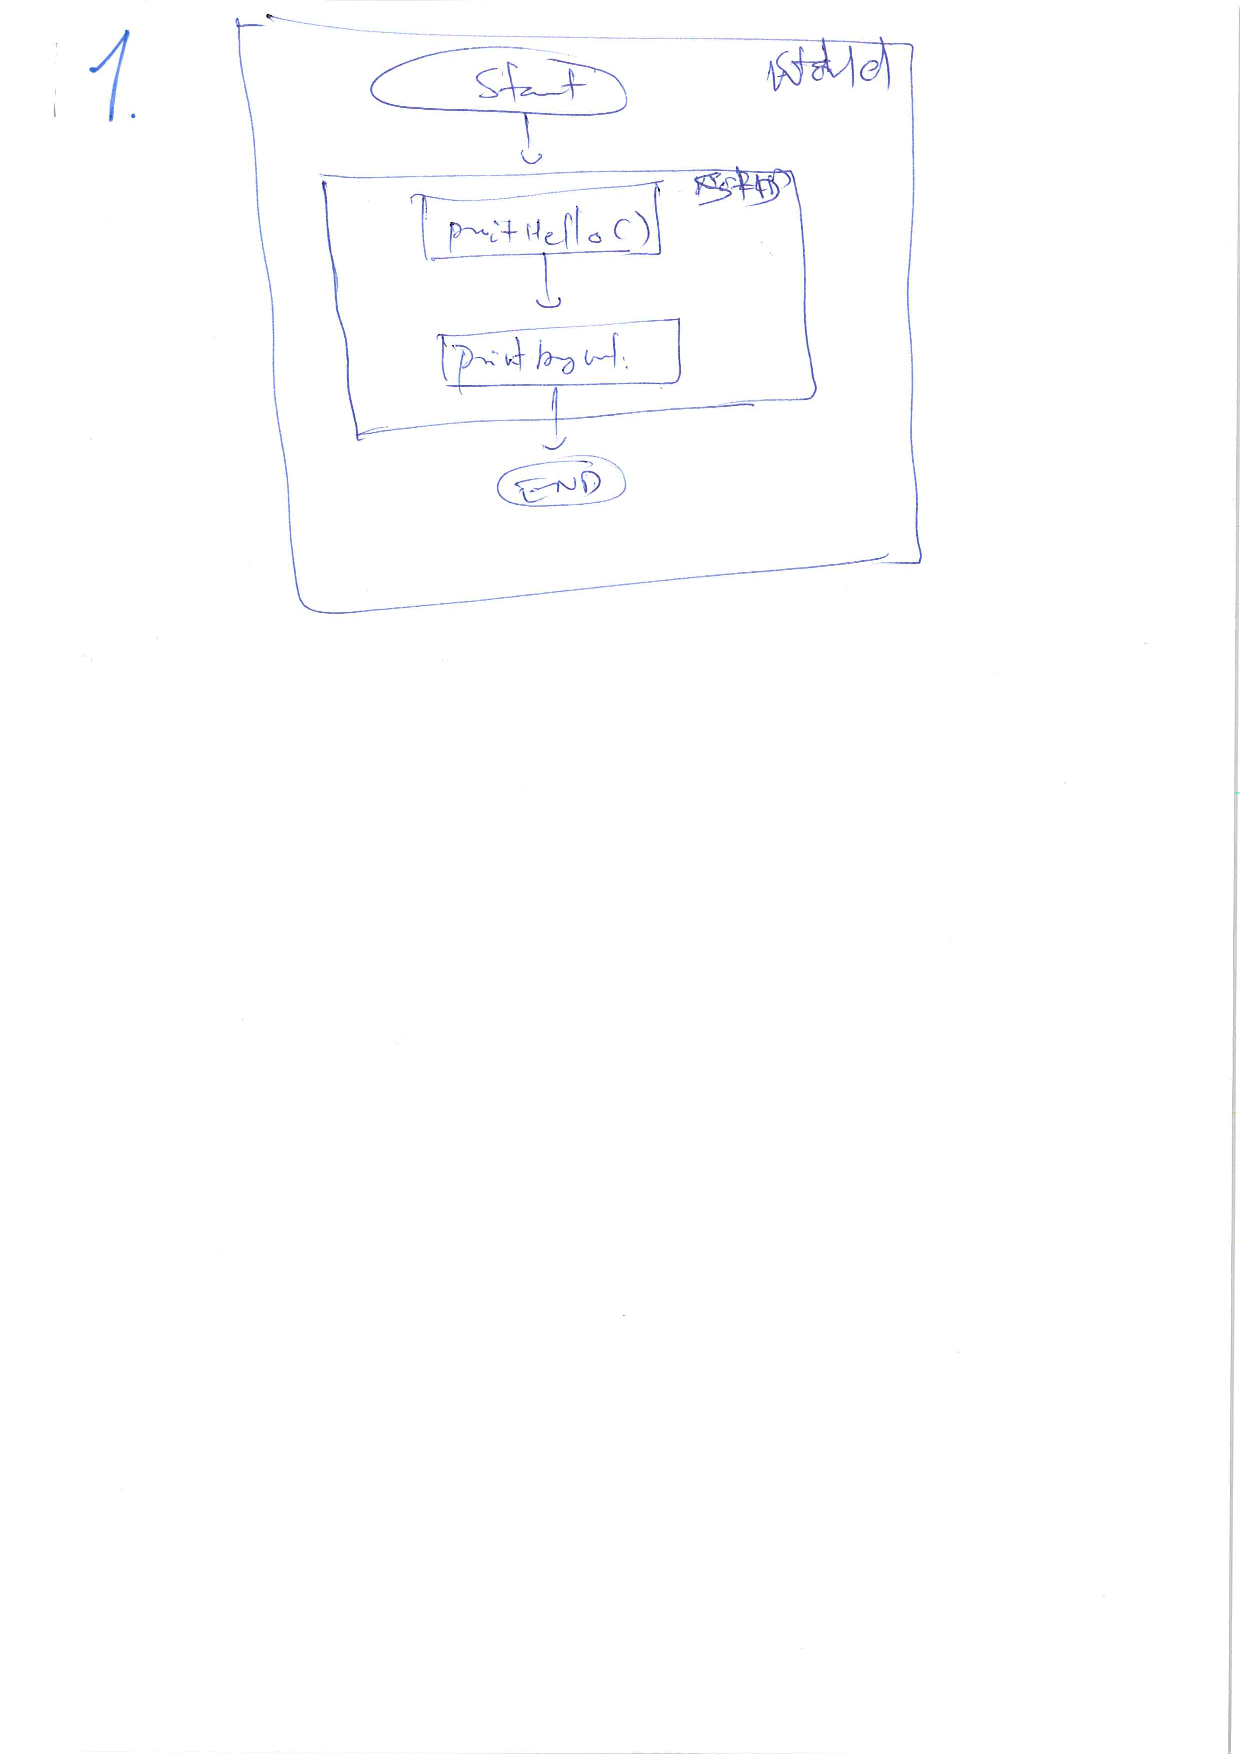
\includepdf[pages={1}]{inc/generalAppendix/userStudies/participantsVisualization.pdf}
\end{itemize}{}
